\newpage
\section{Segmentação Panóptica}
\label{panoptic:panoptic}
A segmentação panóptica \cite{Kirillov2019a} é uma nova abordagem que caminha em busca da unificação dos métodos avançados de segmentações, sendo eles: segmentação semântica e segmentação de instancias \cite{He2020}, as quais foram descritas \textit{à priori}. Baseado nessa abordagem realiza-se a individualização de objetos e cenas, em que cada pixel das imagens passam a ter um \textit{label} de acordo com a classe do objeto em que o pixel se encontra, assim como um identificador que o diferenciará das demais instancias mapeadas.

Dentre os objetos que podem ser diferenciados pela segmentação panóptica, duas categorias são nomeadas, porquanto o que as diferenciam, basicamente, é a determinação se o objeto é contável (como pessoa, carro, cachorro e afins), o qual  recebe a denominação de \textit{thing}, ou se o objeto é incontável e/ou amorfo (como céu, terrenos, paredes e semelhantes), o qual seria classificado como \textit{stuff} \cite{Kirillov2019a, Liu2019, Mohan2020}. Vale destacar que objetos pertencentes à classificação de \textit{stuff} não recebem um identificador, pelo fato de ser impossível conta-los ou distingui-los.

Além disso, no trabalho desenvolvido por \cite{Kirillov2019a}, ficou claro que a rede teve dificuldades para realizar a segmentação de objetos pequenos, todavia estes resultados não são discrepantes na maioria das vezes, quando comparados as segmentações realizadas por humanos, embora os resultados humanos sejam superiores quando quantificados por métricas de \textit{Panoptic Quality} (PQ), \textit{Segmentation Quality} (SQ) e \textit{Recognition Quality} (RQ), em bases de dados que serão discorridas na seção \ref{panoptic:dataset}, como é possível observar na tabela \ref{panoptic:table:1} \cite{Kirillov2019a}.

\begin{table}[!ht]
    \centering
    \caption{\textit{Human vs. machine performance.}}
    \label{panoptic:table:1}
    \begin{tabular}{@{}l|lll@{}}
    \textbf{Cityscape} & PQ   & SQ   & RQ   \\ \hline
    human              & $69.6^{\substack{+2.5\\-2.7}}$ & $84.1^{\substack{+0.8\\-0.8}}$ &  $82.0^{\substack{+2.7\\-2.9}}$ \\
    machine            & 61.2 & 80.9 & 74.4 \vspace*{0.3cm}\\
    \textbf{ADE20k}    & PQ   & SQ   & RQ   \\ \hline
    human              & $67.6^{\substack{+2.0\\-2.0}}$ & $85.7^{\substack{+0.6\\-0.6}}$ & $78.6^{\substack{+2.1\\-2.1}}$ \\
    machine            & 35.6 & 74.4 & 43.2 \vspace*{0.3cm}\\
    \textbf{Vistas}    & PQ   & SQ   & RQ   \\ \hline
    human              & $57.7^{\substack{+1.9\\-2.0}}$ & $79.7^{\substack{+0.8\\-0.7}}$ & $71.6^{\substack{+2.2\\-2.3}}$ \\
    machine            & 38.3 & 73.6 & 47.7
    \end{tabular}

    \vspace*{1 cm}
    Fonte: retirado e adaptado de \cite{Kirillov2019a}.
\end{table}

A partir da imagem \ref{panoptic:fig:1} é possível observar as diferenciações realizadas entre as segmentações de instancias (\ref{panoptic:fig:1}\subref{panoptic:fig:1.1}), contando apenas com o encontro de objetos, a segmentação semântica (\ref{panoptic:fig:1}\subref{panoptic:fig:1.2}), compreendendo classes para cada pixel, mas não diferenciando instancias e, por fim, a segmentação panóptica (\ref{panoptic:fig:1}\subref{panoptic:fig:1.3}) abrangendo \textit{things} e \textit{stuffs}, separando cada uma das instancias, assim como determinando uma classe para cada pixel.

\begin{figure}[H]
   \caption{Segmentações modernas.}
   \centering
   \label{panoptic:fig:1}
    \begin{subfigure}[t]{0.45\textwidth}
        \centering
        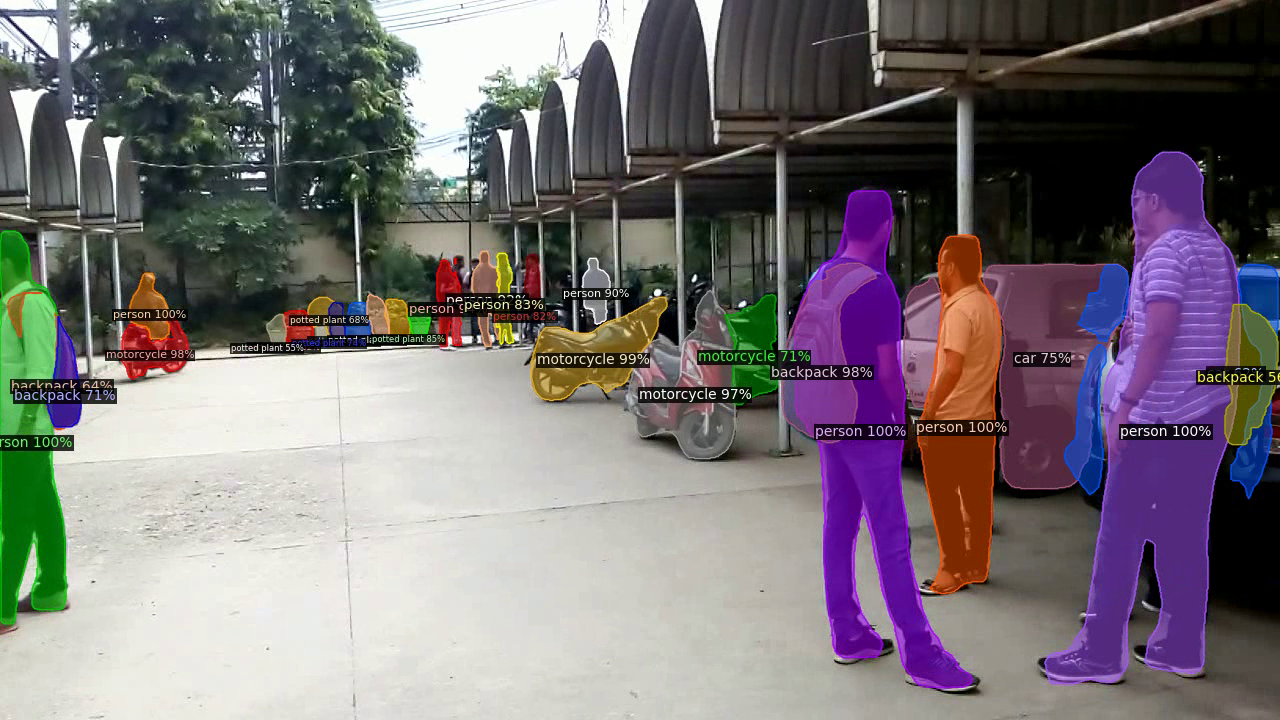
\includegraphics[height=1.5in]{recursos/imagens/panoptic/college_instance.png}
        \caption{Segmentação de instancia.}
        \label{panoptic:fig:1.1}
    \end{subfigure}%
    ~ 
    \begin{subfigure}[t]{0.45\textwidth}
        \centering
        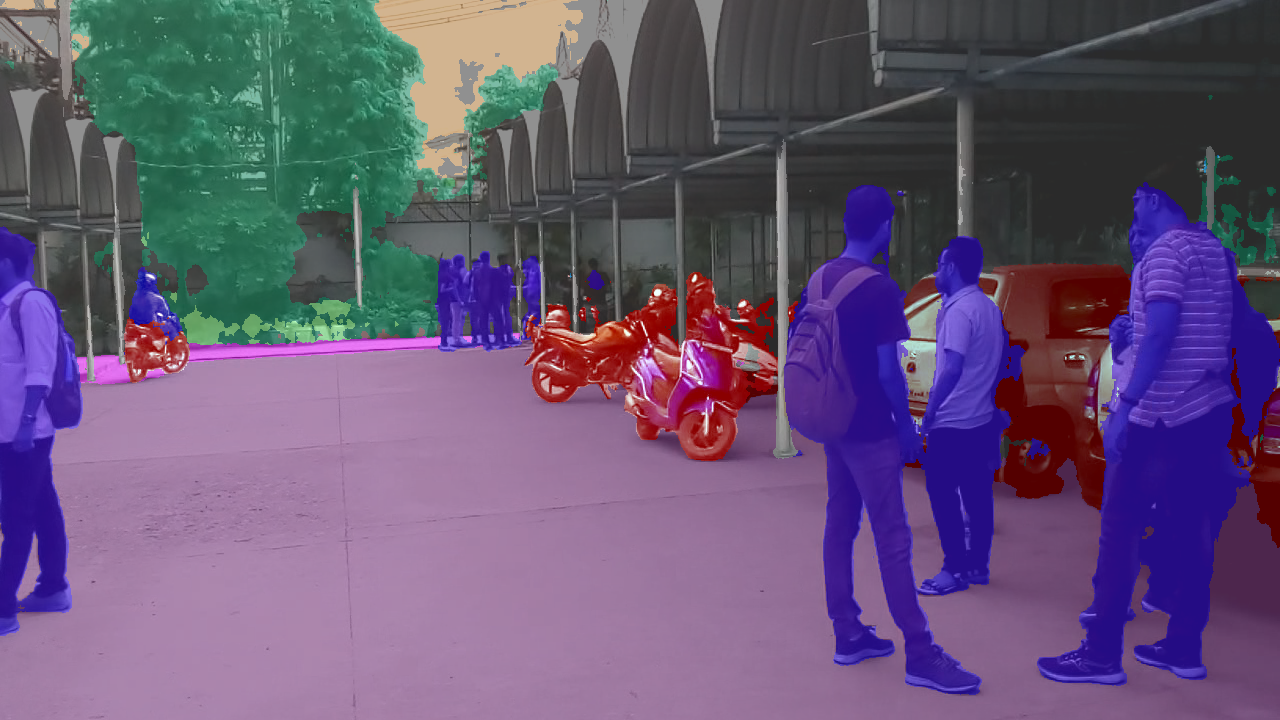
\includegraphics[height=1.5in]{recursos/imagens/panoptic/college_semantic.png}
        \caption{Segmentação semântica.}
        \label{panoptic:fig:1.2}
    \end{subfigure}%
    ~ 
    
    \begin{subfigure}[t]{0.7\textwidth}
        \centering
        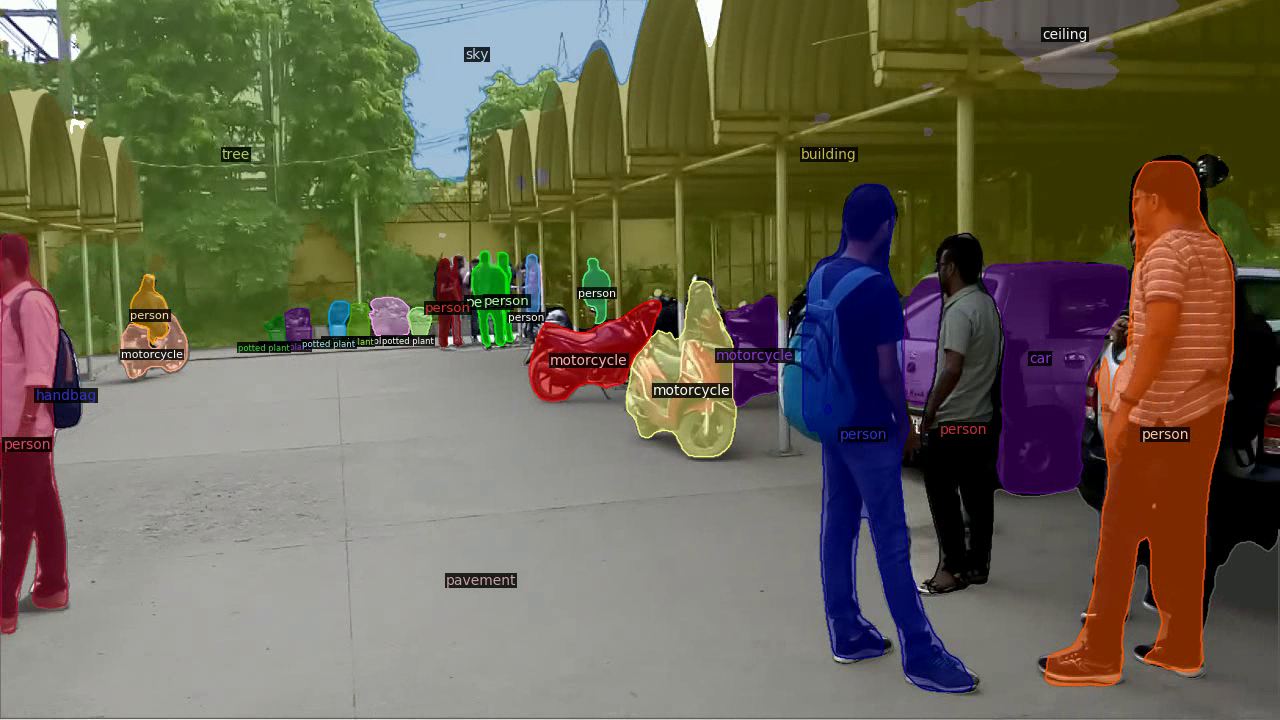
\includegraphics[width=1\linewidth]{recursos/imagens/panoptic/college_panoptic.png}
        \caption{Segmentação panóptica.}
        \label{panoptic:fig:1.3}
    \end{subfigure}

    \vspace*{1 cm}
    Fonte: retirado e adaptado de \cite{2019IntroductionTutorial}.
\end{figure}

Destarte, a segmentação panóptica caminha contribuindo para os avanços tecnológicos em relação ao entendimento de cenários, carros autônomos \cite{Liu2019} e outras situações em que todos os objetos possuem uma determinada relevância no contexto, como realizado em \cite{Brunger2020} que trabalha com a segmentação panóptica de porcos em chiqueiros.

\subsection{Bases de dados}
\label{panoptic:dataset}
Mesmo com a amplitude de \textit{datasets} disponíveis para segmentação de imagens, no âmbito da segmentação panóptica faz-se necessário um cuidado para a escolha dos mesmos, visto que dentre os requisitos necessários, encontra-se a necessidade de anotação dos pixeis e uma identificação das diferentes instâncias, de modo que seja possível diferenciar \textit{things} e \textit{stuffs}.

Dentre os \textit{datasets} trabalhados inicialmente por Kirillov \textit{et al.} \cite{Kirillov2019a}, vale destacar que três possuíam os requisitos necessários, concernindo ao Cityscapes \cite{Cordts2016}, ADE20k \cite{Zhou2016} e Mapillary Vistas \cite{Neuhold2017_ICCV}, mas destacando também a possibilidade de realizar um trabalho com COCO \cite{Lin2014} que havia sido anotada recentemente \cite{Kirillov2019a}.

Após este trabalho, outros \textit{datasets} relacionados a segmentação panóptica foram desenvolvidos, dos quais é possível citar o trabalho de Mohan e Valada \cite{Mohan2020}, que acrescentou os \textit{datasets} KITTI \cite{Geiger2013} e Indian Driving Dataset (IDD) \cite{Varma2018} ao seu trabalho.

Outra opção de \textit{datasets} consiste em uma implementação e uso de uma base de dados interna, como realizado no trabalho de Xiong \textit{et al.} \cite{Xiong2019}, que fez algo similar ao Cityscapes e obteve comportamentos parecidos quanto ao mesmo ou ao do COCO.

De modo geral, a maior parte dos trabalhos realizados consistem em trabalhos com imagens de cidades, carros, metrópoles e afins, como é possível observar na figura \ref{panoptic:fig:3}. Os \textit{datasets} mais populares, logo, aqueles em que há uma preferência na escolha são COCO \cite{Caesar2016, Lin2014} e Cityscape \cite{Cordts2016}, como ocorre nos trabalhos \cite{Chen2019, DeGeus2019a, DeGeus2019, Hou2019, Liu2019, Xiong2019}. Vale frisar que as exceções quanto aos conteúdos dos \textit{datasets} também são encontradas em trabalhos de específicos ou datasets privados, como ocorre no trabalhos desenvolvido por Brünger \textit{et al.} \cite{Brunger2020}.

\begin{figure}[H]
   \caption{Imagens de \textit{datasets} de segmentação panóptica.}
   \centering
   \label{panoptic:fig:3}
    \begin{subfigure}[t]{0.55\textwidth}
        \centering
        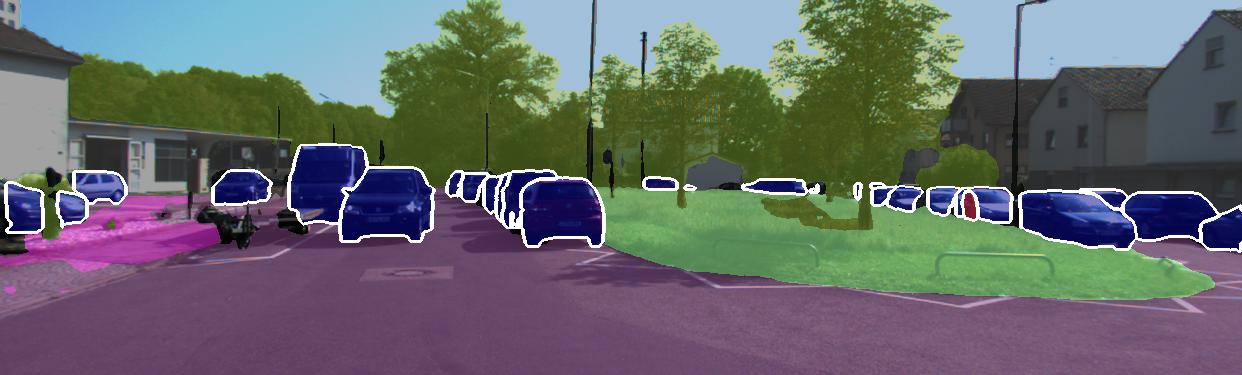
\includegraphics[height=1in]{recursos/imagens/panoptic/kitti.jpg}
        \caption{Imagem do KITTI \cite{Geiger2013}.}
        \label{panoptic:fig:3.1}
    \end{subfigure}%
    ~ 
    \begin{subfigure}[t]{0.45\textwidth}
        \centering
        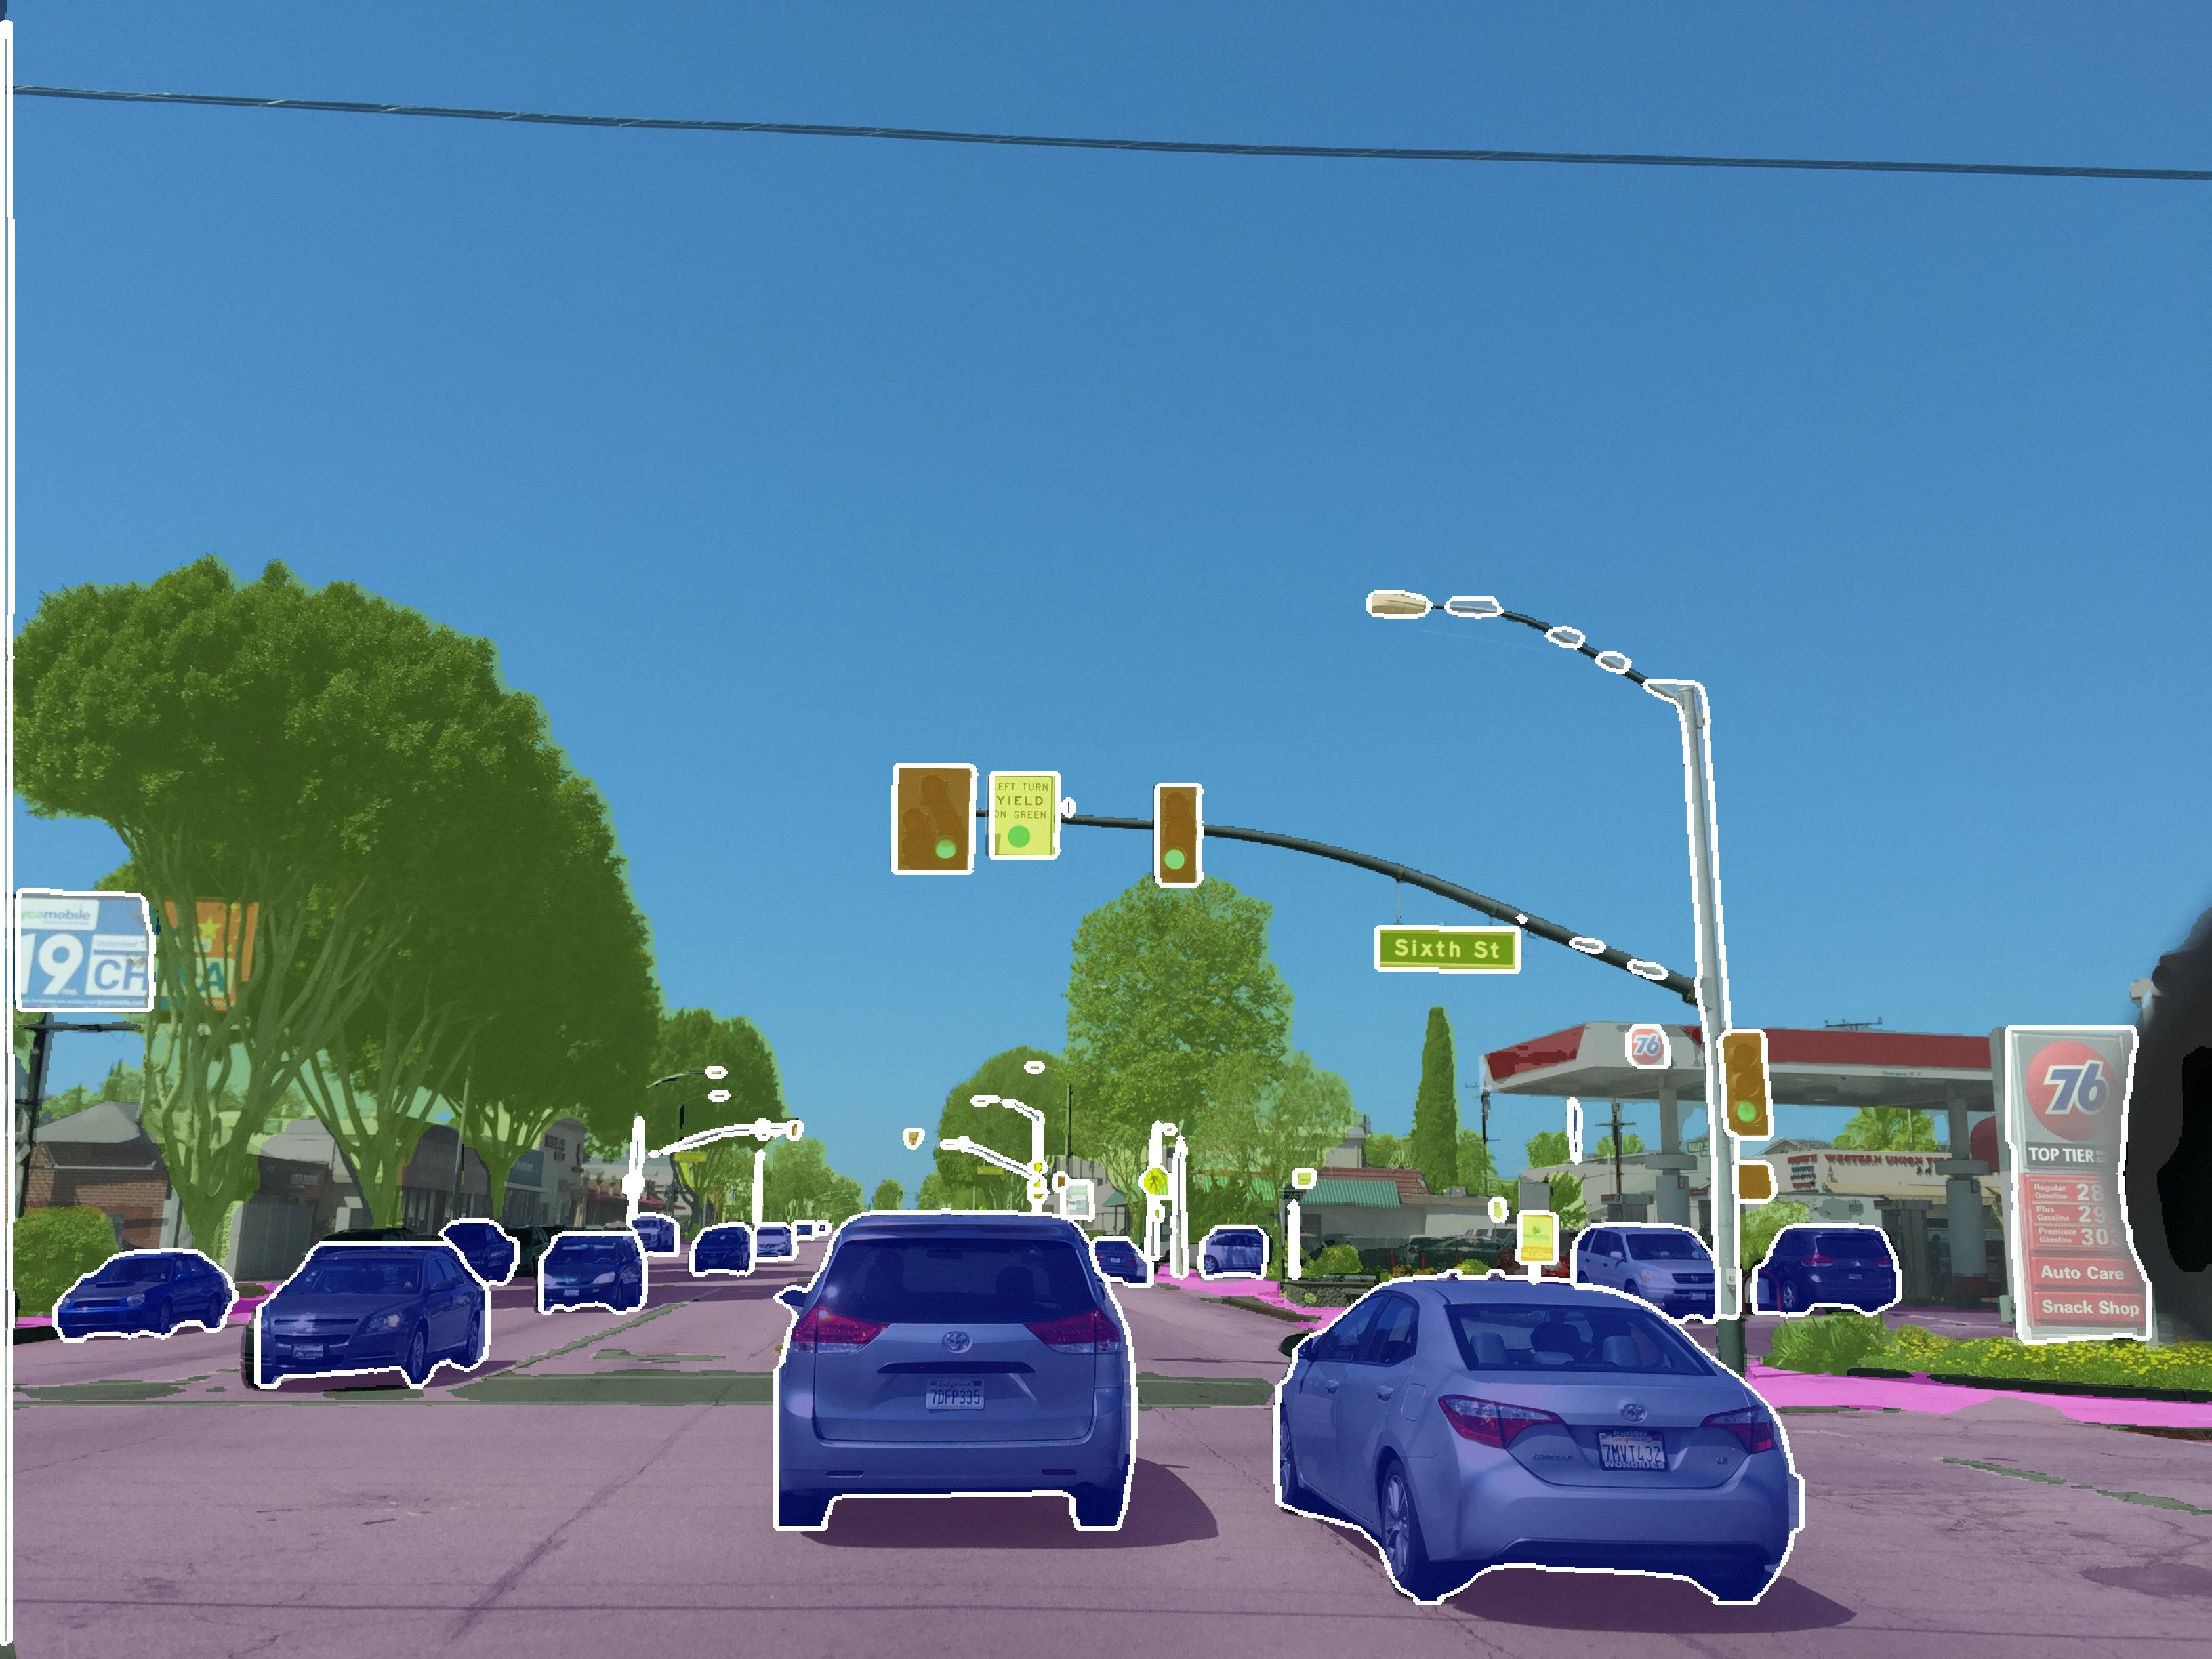
\includegraphics[height=1.3in]{recursos/imagens/panoptic/vistas.jpg}
        \caption{Imagem do Mapillary Vistas \cite{Neuhold2017_ICCV}.}
        \label{panoptic:fig:3.2}
    \end{subfigure}%
    ~ 
    
    \begin{subfigure}[t]{0.45\textwidth}
        \centering
        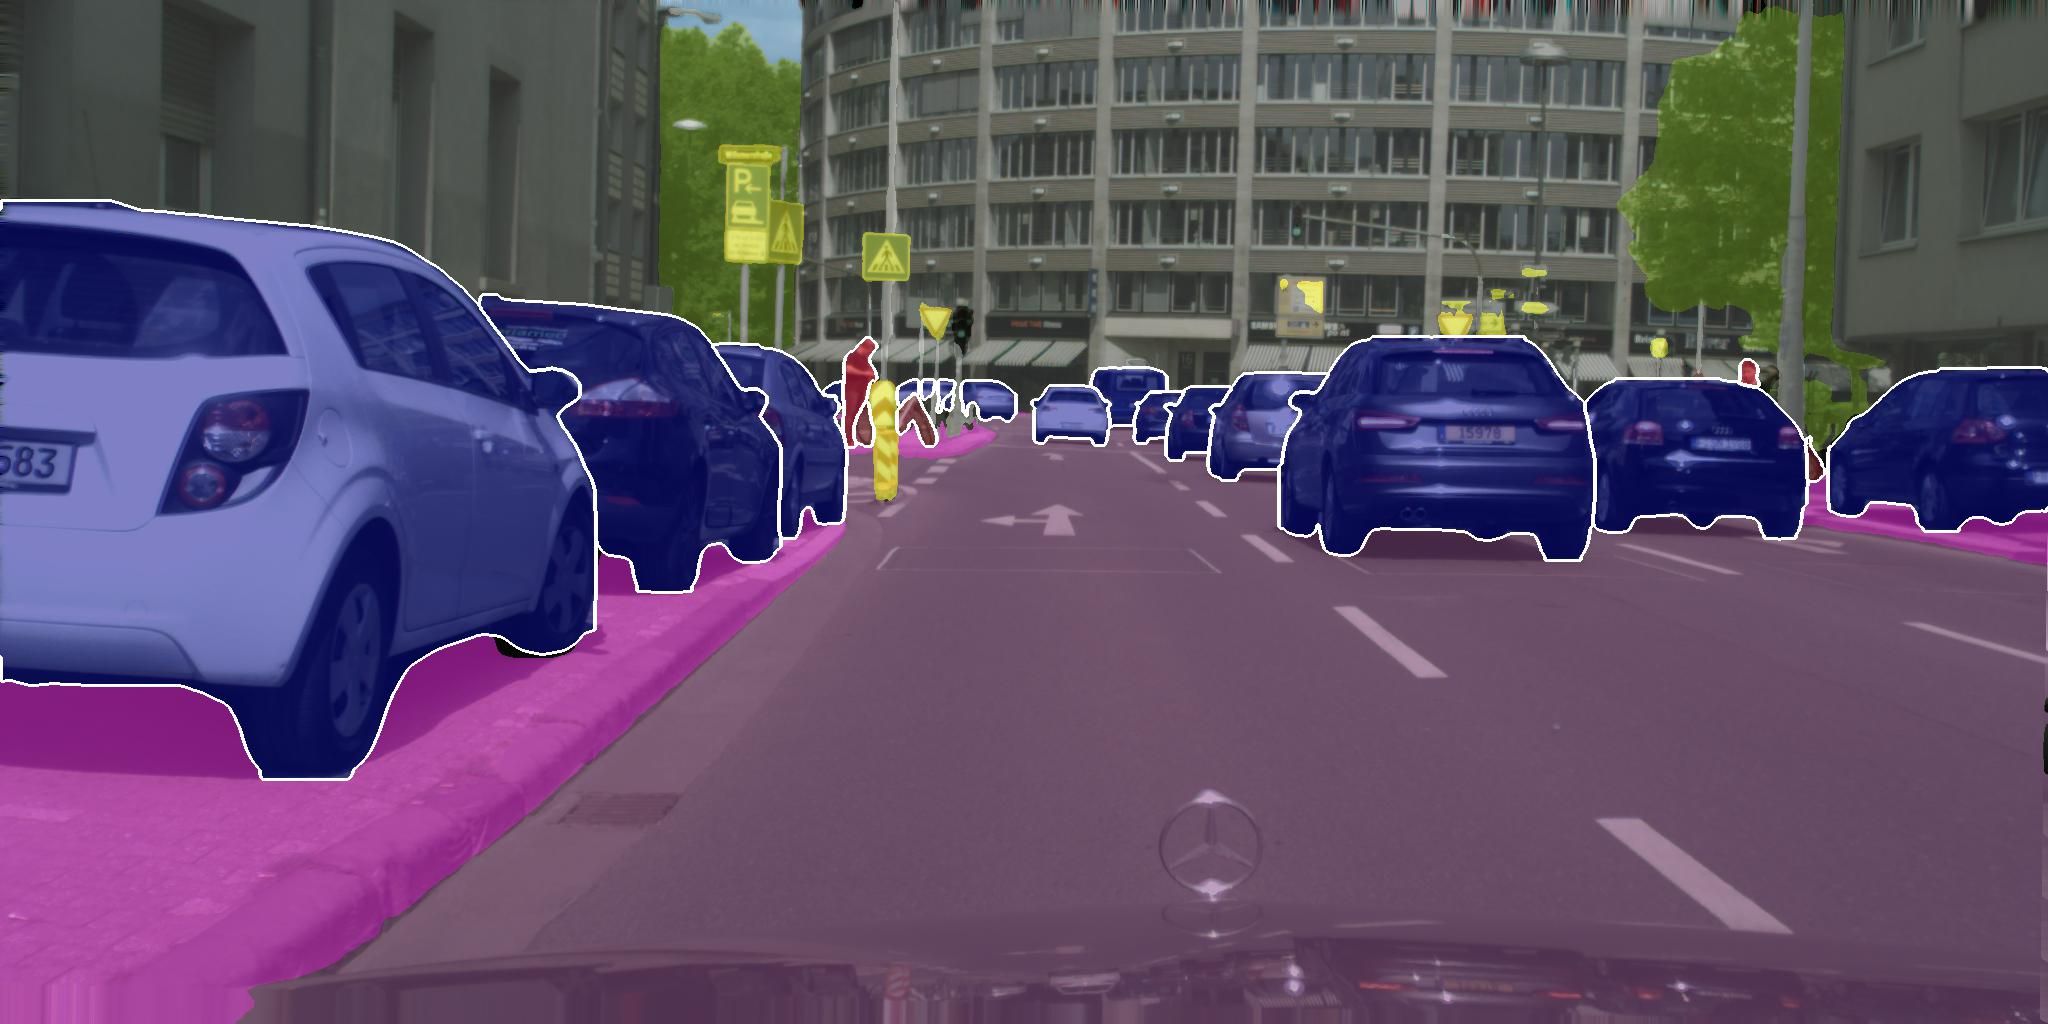
\includegraphics[height=1.3in]{recursos/imagens/panoptic/cityscapes.jpg}
        \caption{Imagem do Cityscapes \cite{Cordts2016}.}
        \label{panoptic:fig:3.3}
    \end{subfigure}
    ~
    \begin{subfigure}[t]{0.45\textwidth}
        \centering
        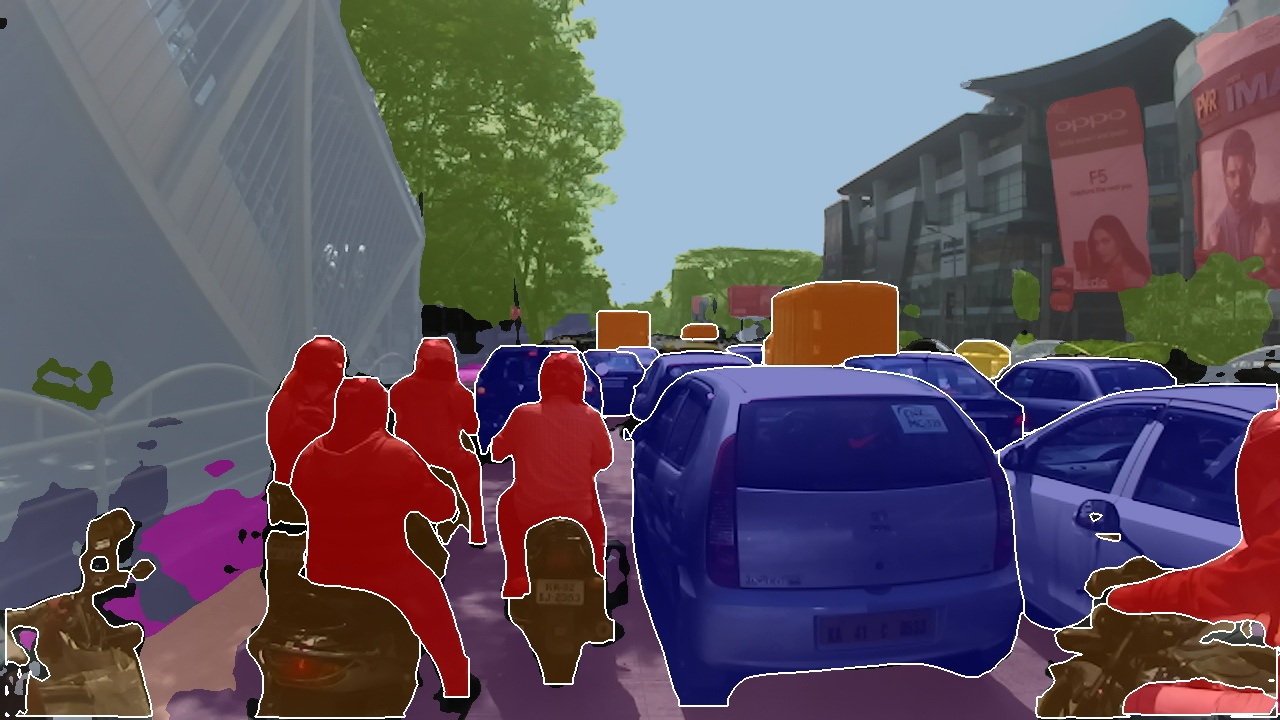
\includegraphics[height=1.3in]{recursos/imagens/panoptic/idd.jpg}
        \caption{Imagem do IDD \cite{Varma2018}.}
        \label{panoptic:fig:3.4}
    \end{subfigure}

    \vspace*{1 cm}
    Fonte: retirado e adaptado de \cite{Mohan2020}.
\end{figure}

\subsection{Arquitetura}
A arquitetura para a formação do modelo de segmentação panóptica, surgiu em um primeiro momento como proposta desenvolvida por Kirillov \textit{et al.} \cite{Kirillov2019a}, de modo que a comportava duas redes. A primeira das redes tinha o objetivo de realizar a segmentação de instancias e essa rede era a Mask R-CNN \cite{He2020}. A segunda rede, por sua vez, seria responsável pela realização da segmentação semântica, em que dentre as testadas o destaque foi para a rede PSPNet multi-scale \cite{Zhao2017}. A proposta do uso dessas redes dava forma para uma arquitetura robusta e poderosa \cite{Kirillov2019a} por trabalhar com redes consideradas estado da arte para a época.

Todavia, após o termino da primeira rede para a realização de segmentação panóptica, outros trabalhos foram realizados, de modo que estes sugeriam novas configurações e levantamentos de pontos diferentes para cada individualidade das configurações adotadas.

Em relação ao desenvolvedor da rede prógona, após os avanços de seus estudos, Kirilovv \textit{et al.} \cite{Kirillov2019} desenvolveu uma arquitetura que propunha a unificação de redes, sendo composta por uma rede Mask R-CNN com uma \hyperref[semantic:FCN]{FCN}, de sorte que esta unificação proporcionasse efetividade para a segmentação de instancias e leveza para a segmentação semântica, mas sem perdas em relação ao seu potencial da rede desenvolvida em seu trabalho anterior, segundo \cite{Kirillov2019}. Para realizar a junção dessas redes foi utilizado dos conceitos e estruturas de uma \textit{Feature Pyramid Network} (FPN) \cite{Lin2016}, um extrator de \textit{features} comum para quem deseja acurácia e desempenhos relevantes não só em relação a grandes objetos, mas também aos pequenos \cite{Lin2016} e assim suprindo uma das desvantagens pendentes na primeira configuração de arquitetura das redes para segmentação panóptica \cite{Kirillov2019, Kirillov2019a}. Destaca-se, ainda, que esta arquitetura com rede FPN trabalha com uma configuração \textit{top-down} com conexões laterais, de modo que torna-se possível realizar uma restauração das resoluções com valorosas informações semânticas. As representações de extração de características com estratégia \textit{bottom-up} e a adotada pela FPN - com conexões laterais - podem ser observadas na figura \ref{panoptic:fig:2}, respectivamente.

\begin{figure}[H]
   \caption{Extrações de características e FPN.}
   \centering
   \label{panoptic:fig:2}
    \begin{subfigure}[t]{0.45\textwidth}
        \centering
        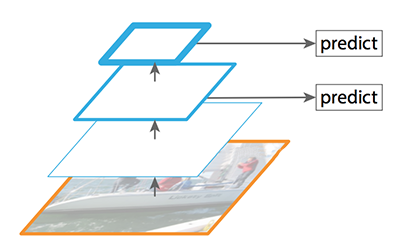
\includegraphics[height=1in]{recursos/imagens/panoptic/bottom-up.png}
        \caption{Configuração \textit{bottom-up}.}
        \label{panoptic:fig:2.1}
    \end{subfigure}%
    ~ 
    \begin{subfigure}[t]{0.45\textwidth}
        \centering
        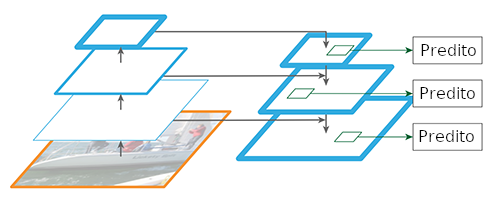
\includegraphics[height=1in]{recursos/imagens/panoptic/FPN.png}
        \caption{FPN.}
        \label{panoptic:fig:2.2}
    \end{subfigure}%

    \vspace*{1 cm}
    Fonte: retirado e adaptado de \cite{Lin2016}.
\end{figure}


\subsection{Métricas}
\label{panoptic:metrics}
Em relação às métricas disponíveis para a avaliação de segmentações panópticas, vale ressaltar que em trabalhos anteriores aos desenvolvidos por Kirillov \textit{et al.} \cite{Kirillov2019a}, a realização da avaliação de \textit{things} e \textit{stuffs} era feita de modo distinto e independente (como \cite{Sun2014, Yao2012}), todavia com uma proposta que disponibilizasse o trato igualitário para os dois tipos de classificação, significado claro, além de fácil entendimento e implementação , Kirillov \textit{et al.} \cite{Kirillov2019a} elaborou o método de \textbf{\textit{Panoptic Quality} (PQ)} que mensurava a qualidade da segmentação realizada em relação ao \textit{ground truth}, que se efetivava  a partir da realização de dois requisitos: 1) encontro de segmentação e  2) calculo de PQ.

A primeira das necessidades é cumprida apenas em segmentações que contam com técnicas de \textit{non-overlapping} para que seja possível encontrar uma única segmentação, como \cite{Neubeck2006}, e possuem um valor de \hyperref[semantic:IoU]{IoU} superior ou igual à 50\% da área em relação ao \textit{ground truth}, sendo esse valor adequado como parâmetro de limiar, sem que ofereça falsas segmentações e consiga trabalhar tanto com objetos grandes quanto com objetos pequenos, segundo \cite{Kirillov2019a}.

Depois, a segunda das necessidades para a determinação de PQ conta com formulas que sugerem a unificação de métricas de SQ e RQ. Além disso, para a determinação dessa formula, faz-se necessário o uso de parâmetros que determinarão segmentações condizentes com o \textit{ground truth}, segmentações não encontradas em relação aos preditos e segmentações não encontradas em relação ao \textit{ground truth}, respectivamente sendo representados por verdadeiro positivo (VP), falsos positivos (FP) e falsos negativos (FN). Logo, a formula para determinação de PQ \cite{Kirillov2019a}, em que $p$ representa os preditos e $g$ representa o \textit{ground truth}, pode ser expressa por:

\begin{equation}
\label{panoptic:eq:1}
    PQ = \frac{\sum _{(p,g) \in VP} IoU(p,g)}{|VP|+ \frac{1}{2}|FP| + \frac{1}{2}|FN|}
\end{equation}

O que remete, também, a uma multiplicação de métrica de qualidade para segmentação por métrica de qualidade para reconhecimento, quando dividida pela quantidade de classificações demarcadas como VP, podendo ser representada por uma segunda formula (\ref{panoptic:eq:2}), como sugere Kirillov \textit{et al.} \cite{Kirillov2019a}.

\begin{equation}
\label{panoptic:eq:2}
   PQ = \underbrace{\frac{\sum _{(p,g) \in VP} IoU(p,g)}{|VP|}}_{SQ} \times \underbrace{\frac{|VP|}{|VP|+ \frac{1}{2}|FP| + \frac{1}{2}|FN|}}_{RQ}
\end{equation}

Assim, com a unificação desses parâmetros e formação da PQ, vantagens podem ser observadas quando comparada a métricas de AP (\ref{instance:AP}), por exemplo, que não podem ser utilizadas para segmentações semânticas, ou quando comparadas a métricas de IoU (\ref{semantic:IoU}) que não pode avaliar corretamente classes do tipo \textit{thing}.

Por fim, vale realçar que uma segunda métrica foi desenvolvida para quantificar segmentações panópticas, sendo esta desenvolvida e disponibilizada de modo \textit{open-source} por \cite{Yang2019DeeperLab:Parser}, que a nomeou de \textit{Parsing Covering}(PQ) e teve iniciativa a partir do trabalho realizado por \cite{Arbelaez2011ContourSegmentation}. A PQ, no que lhe concerne, é uma métrica que não ignora a dificuldade comumente encontrada em redes de segmentação panóptica e concede valor aos tamanhos dos objetos de uma cena, visto que a dificuldade supracitada está na detecção de objetos pequenos. Dessa forma a formula dessa métrica pode ser definida como:

\begin{equation}
    \label{panoptic:eq:3}
    PC = \frac{1}{C} \underset{i=1}{\overset{C}{\sum}}Cov_i
\end{equation}

sendo,

\begin{equation}
    \label{panoptic:eq:4}
    Cov_i = \frac{1}{N_i}\underset{p \in S_i}{\sum} |p|\cdot \underset{g \in S'_i}{max IoU(p,g)}
\end{equation}

\begin{equation}
    \label{panoptic:eq:5}
    N_i = \underset{p \in S_i}{\sum} |p|
\end{equation}

Destarte, quanto ao algarismos desconhecidos, $C$ está relacionado a quantidade de classes semânticas, $S'_i$ e $S_i$ são os valores de segmentação predita e de \textit{ground truth}, respectivamente, $N_i$ representa a quantidade de pixeis de \textit{ground truth} dentro de $S'_i$, $Con_i$ é a classe coberta pela interação e, finalmente, $PC$ é o valor da métrica estabelecido pela média de $Cov_i$ sobre $C$ classes semânticas, segundo as definições de \cite{Yang2019DeeperLab:Parser}.


\subsection{Considerações Finais da Seção}
\label{panoptic:conclusion}
 Na seção \ref{panoptic:panoptic} foi possível observar que as segmentações panópticas embora sejam um assunto relativamente novo, visto que o primeiro trabalho foi realizado por Kirilovv \textit{et al.} \cite{Kirillov2019a} em 2019, esse tipo de segmentação oferece diversos desafios que podem evoluir para as contribuições da ciência, dos quais destacam-se:
 \begin{itemize}
     \item Segmentação desalinhada;
     \item Perda de contexto;
     \item Mau alinhamento;
 \end{itemize}

Esses pontos podem ser observados a partir da figura a seguir (figura \ref{panoptic:fig:4}):

\begin{figure}[H]
   \caption{Falhas de segmentações panópticas.}
   \centering
   \label{panoptic:fig:4}
    \begin{subfigure}[t]{0.7\textwidth}
        \centering
        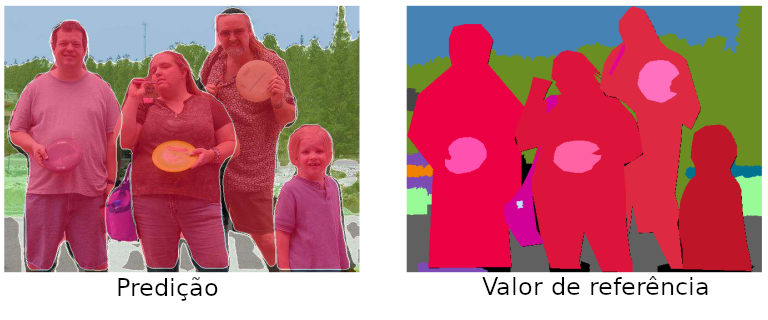
\includegraphics[width=1\linewidth]{recursos/imagens/panoptic/mau_adaptadas.png}
        \caption{Segmentação desalinhada.}
        \label{panoptic:fig:4.1}
    \end{subfigure}%
    ~ 

    \begin{subfigure}[t]{0.7\textwidth}
        \centering
        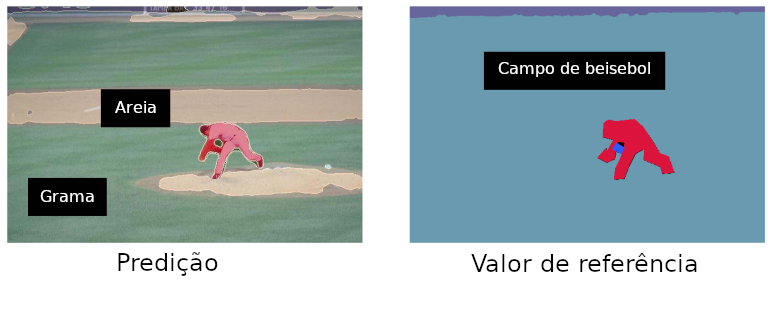
\includegraphics[width=1\linewidth]{recursos/imagens/panoptic/perda_contexto.png}
        \caption{Perda de contexto.}
        \label{panoptic:fig:4.2}
    \end{subfigure}%
    ~ 
    
    \begin{subfigure}[t]{0.7\textwidth}
        \centering
        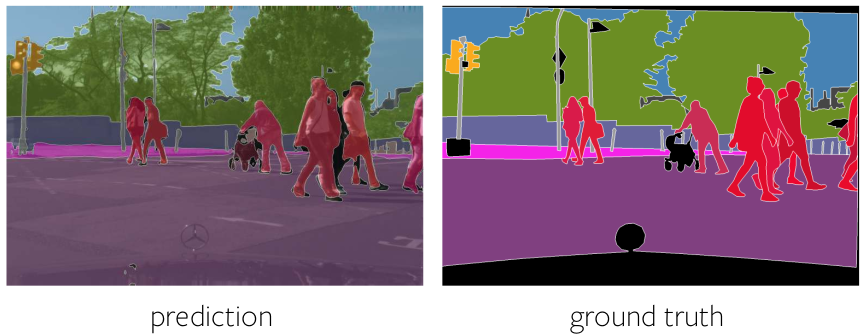
\includegraphics[width=1\linewidth]{recursos/imagens/panoptic/mau_alinhamento.png}
        \caption{Mau alinhamento.}
        \label{panoptic:fig:4.3}
    \end{subfigure}

    \vspace*{1 cm}
    Fonte: \cite{Christoph2019VisualBeyond}.
\end{figure}